\documentclass[10pt,journal,compsoc]{IEEEtran}

\usepackage{grffile}
\usepackage[dvips]{graphicx}

\usepackage[cmex10]{amsmath}

\hyphenation{}

\begin{document}

\title{Eficiencia del sistema de propulsi\'on WARP de la nave espacial USS Enterprise}


\author{Lucila Stancato,~\IEEEmembership{I.T.B.A,}
		Dami\'an Modernell,~\IEEEmembership{I.T.B.A,}
		Juan Brasca,~\IEEEmembership{I.T.B.A,}
		Conrado Negro,~\IEEEmembership{I.T.B.A}%

}

\IEEEcompsoctitleabstractindextext{%
\begin{abstract}
%\boldmath
Analizamos la eficacia en la generaci\'on de n\'umeros pseudoaleatorios del generador de L'Ecuyer aplicando los tests $\chi^2$ y $KS$
, en los que determinamos la conveniencia de usar dicho generador. Utilizando realizaciones de distintas variables pseudoaleatorias,
estimamos el tiempo medio de vuelo de la nave espacial USS Enterprise.
\end{abstract}

\begin{IEEEkeywords}
Generador de L'Ecuyer, n\'umeros pseudoaleatorios, propulsor WARP
\end{IEEEkeywords}
}%\IEEEcompsoctitleabstractindextext

\maketitle

\IEEEdisplaynotcompsoctitleabstractindextext

\IEEEpeerreviewmaketitle

\section{Introducci\'on}

\IEEEPARstart{L}{}os dispositivos de c\'omputo no pueden generar n\'umeros aleatorios dado que 
son dispositivos deterministas. La \'unica manera de obtenerlos ser\'ia a trav\'es de un dispositivo
que detecte procesos naturales como por ejemplo el intervalo de tiempo entre dos part\'iculas $\alpha$
en una muestra radiactiva.\\
En la secci\'on 2 utilizamos y sometemos a prueba el generador propuesto por L'Ecuyer para la
generaci\'on de n\'umeros pseudoaleatorios que a diferencia de los n\'umeros aleatorios, pueden 
ser generados por una computadora. Usamos las pruebas de $\chi^2$ y de Kolmogorov-Smirnov para determinar la bondad de ajuste del
generador. En la secci\'on 3 utilizamos una variable pseudoaleatoria generada con el algoritmo de L'Ecuyer para
obtener variables pseudoaleatorias con distintas funciones de distribuci\'on. En la secci\'on 4 
calculamos la media y la varianza muestral del tiempo de vuelo del USS Enterprise.\\
Comprobamos la efectividad del generador de L'Ecuyer ya que genera n\'umeros que aparentan ser 
aleatorios. ???????????????????????????????????

\section{Generador de L'Ecuyer}
El generador propuesto por L'Ecuyer en 1998 combina dos generadores lineales congruenciales (LCGs).
El algoritmo est\'a compuesto por cinco pasos:
\begin{itemize}
 \item{PASO 1:} Seleccionar una semilla $X_{1,0}$ en el rango $[1,2147483562]$ para el primer LCG y otra $X_{2,0}$ en el rango $[1,2147483398]$ para el segundo LCG.\\
 \item{PASO 2:} Evaluar cada generador individual:
 \begin{align*}
  X_{1,n+1} &= 40014 X_{1,n} mod 2147483563\\
  X_{2,n+1} &= 40692 X_{2,n} mod 2147483399
 \end{align*}
 
 \item{PASO 3:} Computar:
 \begin{equation*}
  X_{n+1} = (X_{1,n+1} - X_{2,n+1}) mod 2147483562
 \end{equation*}
 
 \item{PASO 4:} Computar:
  \begin{equation*}
  \label{eq:f(t)}
  U_{n+1} = \left\{
  \begin{array}{rl}
	\frac{X_{n+1}}{2147483563} \hspace{0.5cm} X_{n+1} > 0\\\\
	\frac{2147483562}{2147483563} \hspace{0.5cm} X_{n+1} = 0\\
  \end{array} \right.
  \end{equation*}

 \item{PASO 5:} Hcer $n = n + 1$ y volver al $PASO 2$
\end{itemize}

Los n\'umeros obtenidos por medio de este generador tienen una distribuci\'on uniforme.
Generamos 10000 n\'umeros pseudoaleatorios con el algoritmo de L'Ecuyer.  Tomamos como semillas $X_{1,0}=23$ y $X_{2,0}=23$, sabiendo que lo importante
es no inicializar al generador con cero.  Una vez obtenidas 10000 realizaciones, las dividimos en 10 intervalos de clase de amplitud uniforme, y 
presentamos las frecuencias obtenidas en el histograma de la figura 1.

\begin{figure}[t]
\label{fig:histogramalecuyer}
\begin{center}
\centering
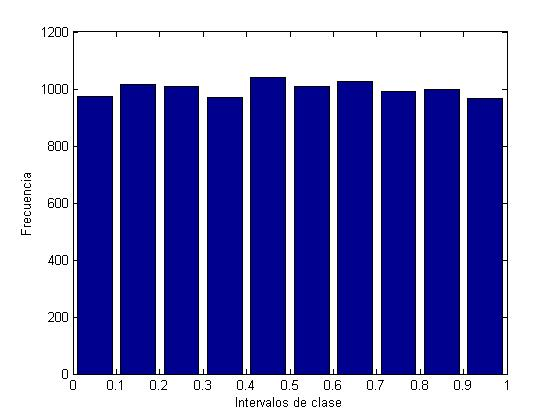
\includegraphics[width=3.2in]{clases.jpg}
\caption{10000 n\'umeros generados con el generador de L'Ecuyer divididos en 10 intervalos de clase que muestran una distribuci\'on uniforme}
\end{center}
\end{figure}


Analizamos gr\'aficamente las realizaciones obtenidas con el algoritmo de L'Ecuyer para analizar la dependencia de una realizaci\'on 
con la anterior.  En la figura 2 mostramos en el plano las duplas $(U_i, U_{i+1})$, que no dejan ver a simple vista los planos de dependecia entre una
iteraci\'on y la siguiente.  En la figura 3 mostramos en el espacio las ternas $(U_i, U_{i+1}, U_{i+2})$, que tampoco evidencian \'areas vac\'ias, o \'areas con mayor concentraci\'on de puntos que otras.


\begin{figure}[t]
\label{fig:2d}
\begin{center}
\centering
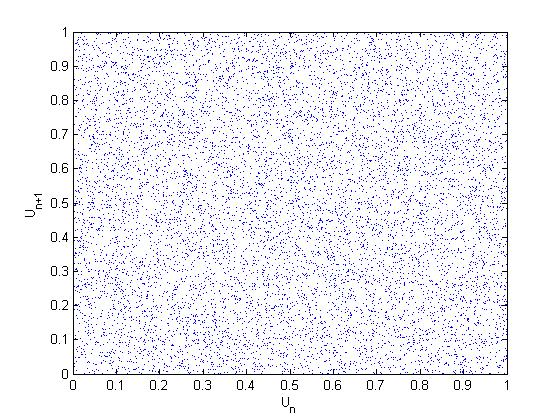
\includegraphics[width=3.2in]{2d_groso.jpg}
\caption{Observamos la distribuci\'on uniforme de los 10000 n\'umeros obtenidos con el generador de L'Ecuyer en el plano}
\end{center}
\end{figure}

\begin{figure}[t]
\label{fig:3d}
\begin{center}
\centering
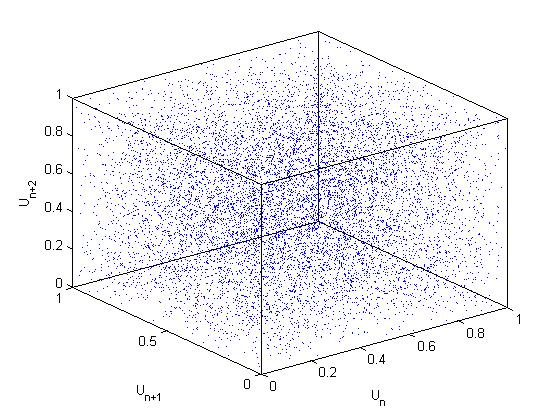
\includegraphics[width=3.2in]{3d.jpg}
\caption{Observamos la distribuci\'on uniforme de los 10000 n\'umeros obtenidos con el generador de L'Ecuyer en el espacio}
\end{center}
\end{figure}

\subsection{Prueba $\chi^2$}
En las figuras 2 y 3 observamos que la distribuci\'on parece ser uniforme, pero podemos usar
tests m\'as elaborados para corroborar esos resultados. El test $\chi^2$ determina, con un nivel
de significaci\'on $\alpha$ (que fijamos en $5\%$) si es razonable suponer que la distribuci\'on 
observada de las 10000 muestras es consistente con que la variable tenga una distribuci\'on uniforme.
Las hip\'otesis del test son:
\begin{itemize}
 \item {$H_{0}$:} $\chi_{0}^2 < \chi_{n-1,\alpha}$ (Los n\'umeros obtenidos mediante el m\'etodo de L'Ecuyer est\'an uniformemente distribuidos)
 \item {$H_{1}$:} $\chi_{0}^2 \ge \chi_{n-1,\alpha}$ (Los n\'umeros obtenidos mediante el m\'etodo de L'Ecuyer no est\'an uniformemente distribuidos)
\end{itemize}
Para la prueba decidimos tomar 10 intervalos de clase, determinando as\'i 9 grados de libertad. Para estos
par\'ametros, obtenemos de tablas el valor cr\'itico $\chi_{n-1,\alpha}^{2} = 16.919$. El estad\'istico $\chi_{0}^{2}$ se computa
mediante la f\'ormula de la ecuaci\'on 1

\begin{equation}
 \chi_{0}^{2} = \sum_{i=1}^{n} \frac{(O_i - E_i)^2}{E_i}
\end{equation}

y resulta $\chi_{0}^{2} = 5.592$ por lo que se acepta la hip\'otesis nula $H_0$.

\subsection{Prueba de Kolmogorov-Smirnov}
Las hip\'otesis utilizadas para esta prueba son:
\begin{itemize}
 \item {$H_{0}$:} $D < D_{\alpha}$ (Los n\'umeros obtenidos mediante el m\'etodo de L'Ecuyer est\'an uniformemente distribuidos)
 \item {$H_{1}$:} $D \ge D_{\alpha}$ (Los n\'umeros obtenidos mediante el m\'etodo de L'Ecuyer no est\'an uniformemente distribuidos)
\end{itemize}
Donde $D$ es el resultado de la prueba y $D_{\alpha}$ es el valor cr\'itico correspondiente a los par\'ametros de la prueba.
Computamos el valor $D$ con la f\'ormula de la ecuaci\'on 2.
\begin{equation}
 D = max(D^{+}, D^{-})
\end{equation}

siendo
\begin{align}
 D^{+} &= max(\frac{i}{n}-x_i)\\
 D^{-} &= max(x_i - \frac{i-1}{n})
\end{align}

donde $x_i$ es el i-\'esimo valor de los calculados por el m\'etodo de L'Ecuyer; 
y el valor $i$ es la cantidad de realizaciones menores que $x_i$ de la muestra de 10000.
Realizando los c\'alculos, resulta $D = 0.0034$ y como $D_{\alpha} = 0.0136$,
 se acepta la hip\'otesis nula.

\section{Generaci\'on de variables aleatorias con distintas funciones de probabilidad}
Teniendo una realizaci\'on de una variable aleatoria con distribuci\'on $U[0,1]$, podemos generar otra variable que tenga
una funci\'on de distribuci\'on $F(x)$. Para hacerlo, calculamos la imagen inversa $x_i = F^{-1}(u_i)$.

\subsection{Distribuci\'on triangular}
La funci\'on de la ecuaci\'on 5 corresponde a la funci\'on densidad de probabilidad de una variable aleatoria con distribuci\'on triangular.
\begin{equation}
   f_{X}(x) = \left\{
  \begin{array}{rl}
	\frac{2(x-a)}{(b-a)(c-a)} \hspace{0.5cm} a \le x \le b\\\\
	\frac{2(c-x)}{(c-b)(c-a)} \hspace{0.5cm} b < x \le c\\\\
	0 \hspace{0.5 cm} Otro \hspace{0.1cm} caso
  \end{array} \right.
\end{equation}


Integramos y calculamos la funci\'on inversa para obtener la expresi\'on de la ecuaci\'on 6

\begin{equation}
 x_i = \left\{
  \begin{array}{rl}
	a+\sqrt{u_i(b-a)(c-a)} \hspace{0.5cm} 0 \le u_i \le \frac{b-a}{c-a}\\\\
	c-\sqrt{(1-u_i)(c-a)(c-b)} \hspace{0.5cm} \frac{b-a}{c-a} < u_i \le 1\\\\
	0 \hspace{0.5 cm} Otro \hspace{0.1cm} caso
  \end{array} \right.
\end{equation}

Aplicamos esta funci\'on de transformaci\'on al set de 10000 valores obtenidos en la seccion 2, y obtenemos
10000 realizaciones de una variable pseudoaleatoria con distribuci\'on triangular.  Dividimos las realizaciones
en 10 intervalos de clase, y graficamos las frecuencias obteniendo el histograma que mostramos en la figura 4.


\begin{figure}[t]
\label{fig:triangular}
\begin{center}
\centering
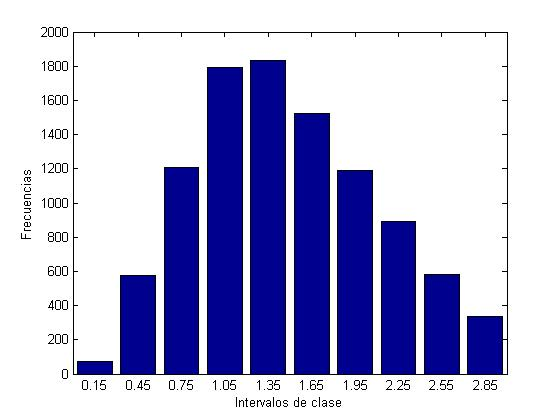
\includegraphics[width=3.2in]{triangular.jpg}
\caption{Histograma de una realizaci\'on de una variable pseudoaleatoria con distribuci\'on de probabilidad triangular con par\'ametros a=0, b=1 y c=3; obtenida a partir de una realizaci\'on de una variable con distribuci\'on uniforme.}
\end{center}
\end{figure}

\subsection{Distribuci\'on exponencial}
La funci\'on de la ecuaci\'on 7 corresponde a la funci\'on densidad de probabilidad de una variable aleatoria con distribuci\'on exponencial.

\begin{equation}
  f_{X}(x) = \left\{
  \begin{array}{rl}
	\lambda e^{-\lambda x} \hspace{0.5cm} 0 \le x\\\\
	0 \hspace{0.5 cm} Otro \hspace{0.1cm} caso
  \end{array} \right.
\end{equation}

Integramos y calculamos la funci\'on inversa para obtener la expresi\'on de la ecuaci\'on 8

\begin{equation}
 x_i = \left\{
  \begin{array}{rl}
	0 \hspace{0.5 cm} u_i = 0\\\\
	-ln(u_i) \hspace{0.5cm} Otro \hspace{0.1cm} caso
  \end{array} \right.
\end{equation}

\subsection{Distribuci\'on uniforme parametrizada}
Para convertir una variable aleatoria con distribuci\'on uniforme $U[0,1]$ en otra variable aleatoria con distribuci\'on
$U[a, b]$, usamos la expresi\'on de la ecuaci\'on 9.

\begin{equation}
 x_i = (b-a)u_i + a
\end{equation}




\section{Estimaci\'on del tiempo de vuelo medio del USS Enterprise}
La nave espacial USS Enterprise, famosa por las pel\'iculas de Star Treck, es impulsada por un sistema de propulsi\'on WARP, 
que se conforma por dos motores a los laterales, uno a babor y otro a estribor. Ambos propulsores son alimentados por un n\'ucleo WARP
donde se llevan a cabo reacciones de aniquilaci\'on materia / antimateria, moderadas por cristales de dilitio. Dichos cristales 
son procesados en una c\'amara controlada, llamada Matriz de Dilitio.\\
El tiempo de operaci\'on de cada propulsor es una variable aleatoria de distribuci\'on exponencial con tiempo medio de 10 d\'ias. 
A su vez, el tiempo de operaci\'on entre fallos del n\'ucleo WARP es de 72 horas, pudiendo variar linealmente hasta en 12 horas. 
La nave puede propulsarse a velocidad WARP con un solo motor funcionando. Por \'ultimo, las c\'amaras de dilitio funcionan de forma tal que, la c\'amara principal tiene un tiempo de operaci\'on entre 
20 y 50 horas, de distribuci\'on uniforme. La c\'amara redundante tiene un tiempo entre fallos de 5 a 12 horas.\\

\indent Definimos dos variables aleatorias  $X_1~U[20,50]$ horas y $X_2~U[5, 12]$, las cuales tienen una distribucui\'on de probabilidad uniforme y corresponden a la c\'amara principal, y a la c\'amara redundante. Tambi\'en definimos una variable aleatoria $X_3$ de distribuci\'on 
triangular, que corresponde al n\'ucleo WARP, con par\'ametros $a = 60$ horas, $b = 72$ horas y $c = 84$ horas. Adem\'as
definimos las variables aleatorias $X_4$ y $X_5$ de distribuci\'on exponencial con $\lambda=1/240$, que corresponden a los propulsores WARP del Enterprise.\\
\indent Para generar las variables pseudoaleatorias $X_1$, $X_2$, $X_3$, $X_4$ y $X_5$ utilizamos 5 variables pseudoaleatorias generadas
a partir del algoritmo de L'Ecuyer.  Para esas 5 variables tomamos 5 semillas distintas (distintas a cero), cuyos valores mostramos en la tabla 1.

\begin{table}[!t]
\renewcommand{\arraystretch}{1.3}
\caption{Semillas de las variables pseudoaleatorias}
\centering
\begin{tabular}{c c}
\hline
\hline
Variable  & Semilla\\
\hline
$u_1$ &  23\\
$u_2$ & 2 \\
$u_3$ & 5 \\
$u_4$ & 17  \\
$u_5$ & 7 \\
\hline
\hline
\end{tabular}
\label{tab:sim}
\end{table}






\begin{figure}[t]
\label{fig:3d}
\begin{center}
\centering
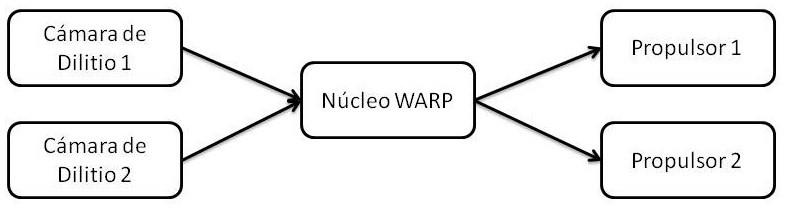
\includegraphics[width=3.2in]{propulsor.jpg}
\caption{Esquema de representaci\'on del sistema de propulsi\'on de la nave espacial USS Enterprise.  La c\'amara de Dilitio 1 es la c\'amara principal, representada por $X_1$. La c\'amara de Dilito 2 es la redundancia, representada por $X_2$. El n\'ucleo WARP est\'a representado
 por $X_3$ y los propulsores estan representados por $X_4$ y $X_5$.}
\end{center}
\end{figure}

Para estimar el tiempo de vuelo del USS Enterprise, definimos una variable aleatoria $T$ que se caracteriza por la ecuaci\'on 10.
\begin{equation}
T = min\{ max\{X_1, X_2\}, X_3, max\{X_4, X_5\} \}
\end{equation}


\indent Estimar el tiempo medio de vuelo con un error porcentual menor al $5\%$, donde el error porcentual se computa
como $100L/\bar{T}$, siendo $L$ la longitud del intervalo de confianza.  Hacemos 279 simulaciones y obtenemos una
media muestral del tiempo de vuelo de $\bar{T}=34.1932$ y un desv\'io muestral de $8.9$.
En la figura 6 mostramos la media muestral en funci\'on de la cantidad de iteraciones realizadas.  Podemos ver que se 
estabiliza mientras m\'as simulaciones se hacen. El desv\'io muestral, que
mostramos en la figura 7 disminuye a medida que aumenta la cantidad de simulaciones.  A su vez, podemos ver en la figura 8,
que el error porcentual, tambi\'en disminuye con la cantidad de iteraciones, y que alcanza un nivel de $5\%$ a las 279 simulaciones.


\begin{figure}[t]
\label{fig:3d}
\begin{center}
\centering
\includegraphics[width=3.2in]{media_muesrtal.jpg}
\caption{Media muestral del tiempo de vuelo en funci\'on de la cantidad de simulaciones.}
\end{center}
\end{figure}


\begin{figure}[t]
\label{fig:3d}
\begin{center}
\centering
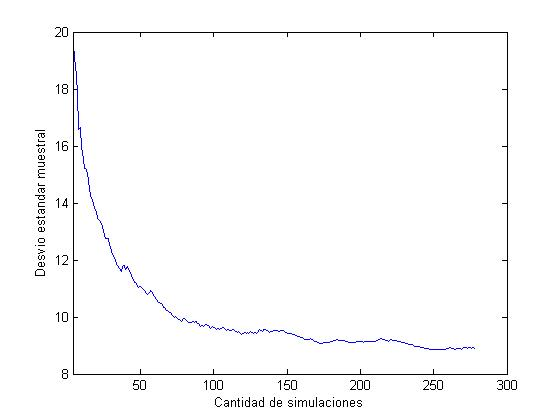
\includegraphics[width=3.2in]{desvio.jpg}
\caption{Desv\'io muestral del tiempo de vuelo en funci\'on de la cantidad de simulaciones.}
\end{center}
\end{figure}



\begin{figure}[t]
\label{fig:3d}
\begin{center}
\centering
\includegraphics[width=3.2in]{error_procentual.jpg}
\caption{Error porcentual del tiempo de vuelo en funci\'on de la cantidad de simulaciones.}
\end{center}
\end{figure}






\section{Conclusi\'on}






\begin{thebibliography}{1}

\bibitem{IEEEhowto:kopka}
D\'iaz, A. R. \emph{El concepto de control}. Departamento de Ingenier\'ia Informatica. 
Instituto Tecnol\'ogico de Buenos Aires.


\bibitem{IEEEhowto:kopka}
Tabla de valores cr\'iticos de la distribuci\'on $\chi^2$. http://www.mat.uda.cl/hsalinas/cursos/2008/probablilidad/Tab\\laChiCuadrada.pdf

\bibitem{IEEhowto:kopka}
Kolmogorov-Smirnov Test. http://www.eridlc.com/onlinetextbook\\/index.cfm?fuseaction=textbook.appendix\&FileName=Table7

\bibitem{IEEhowto:kopka}
Tabla de distribuci\'on T-Student. http://www.dm.uba.ar/materias/\\probabilidades\_estadistica\_C/2008/2/tdist.pdf

\end{thebibliography}

\end{document}


